\documentclass{article}
\usepackage[utf8]{inputenc}
\usepackage[portuguese]{babel}
\usepackage{csquotes}
\usepackage{graphicx}
\usepackage{adjustbox}
\usepackage{lipsum}
\usepackage[backend=biber,autolang=other,
  bibencoding=utf8,style=alphabetic,
  ibidtracker=true]{biblatex}
\addbibresource{suger.bib}

\title{O abade Suger de Saint-Denis}
\date{18 de Janeiro de 2014}
\author{João Távora \\Faculdade de Belas Artes da Universidade de Lisboa}

\begin{document}

\maketitle

\section{Sinopse}

O abade de Suger é uma figura pivotal em França e na Idade Média,
tendo tido uma grande influência nos planos artístico, religioso e
político. O presente trabalho analisa alguns aspectos desta
influência.

\section{Palavras-chave}

Suger, Idade Média

\section{Introdução}

A vida e o legado escrito do abade Suger de Saint-Denis fornecem uma
perspectiva única das motivações e justificações deste Abade do século
XII como patrono de diversas artes. Partindo da posição pouco habitual
de ter sido amigo de infância daquele que viria a ser o rei de França,
Suger promove uma união política importante que une o reino ao Papado
contra o imperador Henrique V, torna-se abade da de Saint Denis e
chega a ser regente do Reino de França.

Os seus relatos dos trabalhos que impulsionou em St. Denis expressam,
nas palavras de Erwin Panofsky, um dos primeiros exemplos da ``grande
excepção à regra, um patrono tornado \emph{littérateur}''
\cite{panofsky-suger}.

Os principais protagonistas do seu tempo, como os reis Luís VI e Luís
VII, Bernardo de Claraval, Pedro Abelardo e o papa Calisto II,
fornecem o pano de fundo político-filosófico para os movimentos
estéticos promovidos por Suger. Estes centraram-se na reforma e
reconstrução da igreja gótica de St. Denis, que viria a ser um
influência determinante na arquitectura e estética em toda a França.

\section{Aspectos biográficos}

As origens da família de Suger são desconhecidas. Por diversas vezes
nos seus escritos, Suger sugere a proveniência de um meio humilde,
embora isso possa ser uma convenção da escrita autobiográfica
\cite{wikipedia-suger}. Em 1091, aos 10 anos de idade, Suger foi
cedido como oblato à abadia de St. Denis, onde principiou a sua
educação, tendo sido mais tarde aprendiz no priorado de Saint-Denis de
lÉstrée. Terá sido aqui que conheceu aquele que viria a ser o rei de
França Luís VI, também conhecido como Luís, o Gordo. Depois de ter
frequentado uma escola vizinha de 1104 até 1106, Suger tornou-se
secretário do abade de St. Denis. Nos ano seguintes, tornou-se
preboste de Berneval na Normandia, e em 1009 de Toury. Em 1118, o rei
de França enviou Suger como conselheiro à corte do Papa Gelásio II, em
Maguelonne, que tinha acabo de regressar a França depois das
turbulências advindas da querela das investiduras papais com o
imperador Henrique V. Suger viveu até 1122 na corte do sucessor de
Gelásio, Calisto II.

No seu regresso, Suger tornou-se abade de Saint-Denis. Até 1127,
ocupou-se principalmente com os assuntos do reino, mas durante a
década seguinte, dedicou-se à reorganização e reforma de St. Denis.

Em 1137, acompanhou aquele que viria a ser o rei Luís VII, também
chamado Luís, o Jovem, até à Aquitânia, na ocasião do casamento desse
príncipe com Leonor de Aquitânia. Na ausência do rei durante a Segunda
Cruzada, de 1147 até 1149, foi regente do reino de França. Este
casamento traria para o Reino de França o vasto condado da
Aquitânia. Até à sua morte, Suger opôs-se à dissolução do casamento, o
que em 1152 acabou por ocorrer pelo mesmo não ter produzido herdeiro.

\section{Política: influência e regência}

Suger tinha a plena na segunda década do século XII a plena confiança
do rei Luís VI, com quem tinha crescido em criança e desempenhava na
sua companhia um papel semelhante ao de um primeiro-ministro.

Numa missão de vulto a cargo de Luís VI, o Gordo, Suger viaja ao
encontro do Papa Gelásio II, em fuga de Roma para França depois de
numa atmosfera turbulenta ter excomungado da Igreja Católica o
imperador do Sacro Império Romano-Germânico Henrique V. Este último
lutava pela manutenção do \emph{Previligium}, ou o direito a nomear os
papas como entendesse. Gelásio II viria a morrer na abadia de Cluny
enquanto tentava convocar um conselho que resolvesse o problema da
investidura papel, algo que só viria a ser conseguido pelo seu
sucessor Calisto II.  Suger tem um papel instrumental na aliança entre
o papado e a França contra o Sacro Império. Em 1124, e na consequência
no conselho de Reims, o imperador decide invadir a França, mas é
obrigado a recuar por uma união forte entre os senhores Feudais
franceses.

Luís VII, sucessor de Luís VI, passou grande parte da sua juventude em
Saint-Denis, onde aprendeu a confiar e a valorizar as opiniões do
abade Suger, que seria um bom conselheiro durante os primeiros anos do
seu reinado.

É Suger quem guia o jovem príncipe à sua futura mulher Leonor de
Aquitânia e a um casamento que traz para o Reino de França a aliança
político-militar do vasto e poderoso condado da Aquitânia. O casal,
cujo casamento só viria anulado depois da morte de Suger, participou
na cerimónia inaugural da Abadia de St. Denis.

Quando Luís VII partiu para a Segunda Cruzada, Suger torna-se regente
do Reino de França, e à chegada do Rei, é nomeado por este ``pére de
la patrie''.

Suger roga a Luís VII que controle as ameaças dos senhores feudais
vizinhos, e simultaneamente é responsável pela estratégia real de
controlo das rebeliões populares contra o mesmo regime
senhorial. Concentrou ainda esforços na regularização do sistema
administrativo da justiça. Suger formula uma teoria da pirâmide de
vassalagem \cite{wikipedia-suger}: o Rei, no topo dessa pirâmide é
considerado ``o primeiro entre pares''. Suger parece expressar já uma
certa ideia de Estado, ao escrever \cite{wikipedia-suger}:

\begin{quote}
Il n’est ni juste ni naturel que l’Angleterre soit soumise aux
Français ou la France aux Anglais.
\end{quote}

Suger está igualmente na origem d''As grande crónicas de França'' que
constitui a história oficial da monarquia francesa e para a qual
redige um primeiro volume dedicado a Luís VI, o Gordo.

\section{Reforma e reconstrução da Abadia de St. Denis}

É no regresso da missão à corte do Papa Gelásio II que Suger é
informado da morte de Adam, abade de St. Denis. É tentada uma eleição
de um novo abade sem o consentimento do soberano. Ao ser alertado,
Luís VI toma imediatamente a medida preventiva de incarcerar os
principais pretendentes \cite{wikipedia-suger}.

Para o rei, os eclesiásticos e as abadias são elementos importantes da
estabilização do poder. Como tal, não é possível deixar ao clero a
liberdade de escolha sem correr um grande risco político num período
de confrontação feudal. A eleição de Suger, um homem próximo do
soberano e, recentemente, do papado exilado, vem criar consenso num
conflito semelhante ao que ocorria com a querela das investiduras
papais, entre as pretensões da igreja a um direito canónico e a
autoridade real.  

Em 1122 os prisioneiros de Luís VI são libertados e Suger é ordenado
abade de St. Denis, com todos os bens e privilégios da Abadia.

Em 1130, impulsionadas por Suger, começam obras de restauração na
abadia que conduzirão a uma considerável ampliação e completa
transformação da arquitectura da abadia. Suger virá mais tarde a
justificar as reparações sublinhando o elevado estado de degradação em
que se encontrava a antiga igreja carolíngia \cite{calado}.

Nos textos que Suger legou não há uma menção clara de quem terá sido o
arquitecto da reconstrução de St. Denis, ficando apenas claro que foi
o próprio Suger quem idealizou a construção.

Os modelos arquitectónicos que inspiraram a reconstrução foram a
grandiosa ``Hagia Sophia'', a igreja do imperador bizantino
Justiniano, bem como o Templo de Salomão em Jerusalém, conhecido
apenas pelos textos bíblicos.

A reconstrução da igreja pode dividir-se em obras da fachada, no coro
e na nave, tendo esta última ficado incompleta. Nas influências
concretas da reconstrução contam-se as da arte da Normandia e
Borgonha. O coro de Saint Denis tem influência das catedrais destas
duas regiões, possuindo um deambulatório com capelas radiantes do tipo
esboçado na \ref{fig:1}.

\begin{figure}
\centering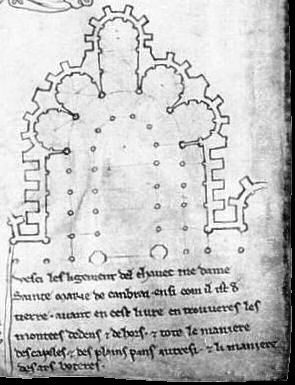
\includegraphics[height=0.6\textheight,keepaspectratio]
                          {images/villard-coro.jpg}
  \caption{Pormenor do caderno de desenhos de Villard de Honnecourt
    esboçando um coro com capelas radiantes}.
  \label{fig:1}
\end{figure}


O prestígio da abadia de St. Denis antes da era de Suger tinha já sido
divulgado por obras literárias como a ``Pélerinage de Charlemagne''
que atribui as relíquias da Paixão de Cristo a Carlos Magno. Segundo a
lenda, teria sido o próprio Cristo a consagrar originalmente a abadia,
e acredita-se que se trata de uma igreja contemporânea com a
cristianização da Gália \cite{wikipedia-abadia}. 

As opções estéticas tomadas por Suger visam continuar a grandiosidade
e relevância sagrada da igreja. Suger dedica também considerável
esforço ao estudo da personagem do santo que dá nome à Abadia, ainda
que assente num curioso equívoco historiográfico.

Sabe-se hoje que St. Denis, o santo, tem raízes reais e místicas
\cite{calado}. Segundo as primeiras, terá sido um mártir que no
séc. III converteu os francos ao cristianismo. No entanto, St. Denis
pode ser também Diosínio, o Areopagita, um teólogo oriental que terá
conhecido o próprio São Paulo, apóstolo de Cristo. A este último foi
atribuído um texto grego que data do séc. V. Dada a discrepância de
quase cinco séculos, a autoria é hoje em dia atribuída àquele que
ficou conhecido como Pseudo-Dionísio Areopagita. No entanto, no séc
VII o Papa envia o documento a Pepino, o Breve, pai de Carlos Magno, e
a partir desse momento St. Denis passa a ser simultaneamente o
conversor dos francos bem como o autor do texto teológico.

O texto viria a inspirar Suger, que pretendia traduzir em linguagem
arquitectónica o pensamento místico de Pseudo-Dionísio Areopagita,
autor neoplatónico do séc. V que Suger julgou ser o verdadeiro patrono
da Abadia. De resto, a estética de Suger é a dos séculos XII e XIII
com tendências platonizantes e influenciada pela obra de Santo
Agostinho de Hipona.

No ``Folheto da Consagração'' que viria a escrever para a cerimónia da
dedicação e consagração da igreja, Suger retoma passagens de
St. Agostinho que comparam a basílica a uma imagem celestial e
relaciona a arte da construção com a edificação espiritual. Segundo
Suger, aqueles que participam na construção são gradualmente
``edificados'', iluminando-se as suas almas pela visão da harmonia
divina reflectida , em todo o seu esplendor, na obra de arte
material. Suger parafraseia ainda a ideia Agostiniana de que a lei da
proporção harmónica, origem da música e que reconcilia a dissonância
do universo, é a origem de toda a beleza. No folheto, é a temática
musical que confere unidade à argumentação, sendo a paz suprema de
Deus profetizada através de uma sinfonia cósmica. A importância dada à
construção de um coro com capelas radiantes, e a sua apropriação para
o canto litúrgico, pretendia sublinhar que o projecto arquitectónico
de St. Denis é o equivalente visual dessa música divina.

A cerimónia de dedicação de St. Denis teve lugar na presença de Luís
VII e da sua mulher Leonor de Aquitânia, bem como de figuras de enorme
poder dentro do clero. A festa visava salientar o vínculo especial
entre o soberano e o St. Denis, patrono de França. Na procissão desta
segunda consagração, Suger pretendia emular a lendária consagração
original de Cristo, colocando o rei de França no centro da mesma, e
desta forma contribuindo decisivamente para a consolidação de França
sob a coroa de Luís VII.

O estilo arquitectónico da nova abadia de St. Denis, que evoca para a
monarquia Francesa os modelos místicos da ordem política, viria a ser
adoptado por todas as catedrais francesas que a sucederam, como Paris,
Chartres, Reims e Amiens.

\begin{figure}
\centering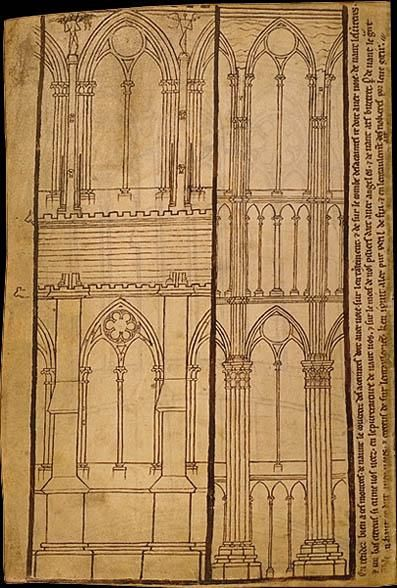
\includegraphics[height=0.6\textheight,keepaspectratio]
                          {images/villard-reims.jpg}
  \caption{Janelas da catedral de Reims do caderno de desenhos de
    Villard de Honnecourt.}.
  \label{fig:2}
\end{figure}

\subsection{Relação com S. Bernardo de Claraval}

O Abade Suger de St. Denis é um defensor dos ornamentos sumptuosos da
igreja. Os autores neo-platónicos que o guiam descrevem a uma ascensão
platónica do sensível ao inteligível, ou do mundo material ao
imaterial. Segundo \cite{panofsky-suger}, a contemplação das pedras
preciosas ou da luz filtrada através dos vitrais das capelas
radiantes leva o abade de Suger a um estado de transe místico.

A descrição que Suger faz de um cálice (\ref{fig:3}), um dos numerosos
vaso litúrgicos encomendados para a Abadia, dá notícia de um critério
estético sensível. Suger fala das ``propriedades das [matizes de cor]
que parecem atravessar-se mutuamente'' \cite{jago-suger}.

\begin{figure}
\centering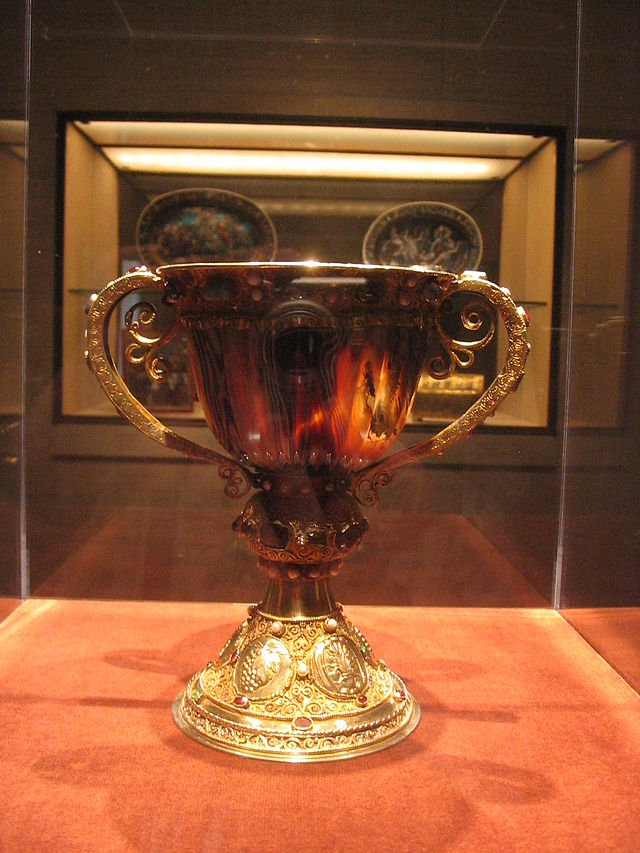
\includegraphics[height=0.6\textheight,keepaspectratio]
                          {images/suger-calice.jpg}
  \caption{Cálice do abade Suger de Saint-Denis.}.
  \label{fig:3}
\end{figure}

Ao gosto pela ornamentação do qual Suger vem dotar a Abadia opõe-se a
à exigência de despojo do ornamento e recusa do luxo, bem como à
eliminação de qualquer figuração que pudesse minar o propósito da
oração. Esta posição foi tomada por Bernardo de Claraval, abade de
Claraval e impulsionador decisivo da expansão da ordem de Cister, que
em \cite{bernard-apologie} faz uma descrição sarcástica do tipo de
Igreja da ordem de Cluny:

\begin{quote}
  L'Église resplendit dans ses murs et elle n'a rien pour ses
  pauvres. Elle revêt d'or ses pierres et abandonne ses fils tout
  nus. Aux dépens des miséreux, on régale les yeux des riches. Les
  curieux trouvent de quoi s'amuser, mais pas les malheureux pour se
  sustenter.

  [...]

  Mais que font dans les cloîtres, devant les frères en train de lire,
  ces grotesques qui prêtent à rire, ces beautés d'une étonnante
  monstruosité ou ces monstres d'une étonnante beauté ?
\end{quote}

E referindo-se possivelmente ao próprio Suger, escreve em
\cite{bernard-critique}:

\begin{quote}
  Il m'est arrivé de voir, c'est la pure vérité, un abbé se faisant
  accompagner de soixante chevaux et plus. Lorsqu'on voit passer cette
  sorte d'abbé, on dirait non pas des gardiens paternels de monastère,
  mais des seigneurs châtelains, non des hommes ayant charge d'âme,
  mais des princes gouvernant des provinces
\end{quote}

Suger responde no ``Folheto da Consagração'' \cite{suger-folheto}, que
ainda que ``uma alma santa e um espírito puro'' sejam fundamentais, se
deve igualmente servir a Deus com os ``ornamentos externos dos vasos
sagrados''. Para Suger, deve-se acompanhar a ``pureza interior'' com
uma ``nobreza exterior''.

\begin{quote}
 Que chacun suive sa propre opinion. Pour moi, je le déclare, ce qui
 m'a paru juste avant tout, c'est que tout ce qu'il y a de plus
 précieux doit servir d'abord à la célébration de la sainte
 eucharistie. Si, selon la parole de Dieu, selon l'ordonnance des
 prophètes, les coupes d'or, les fioles d'or, les petits mortiers d'or
 devaient servir à recueillir le sang des boucs, des veaux et d'une
 génisse rouge, combien d'avantage, pour recevoir le sang de
 Jésus-Christ, convient-il de disposer les vases d'or, les pierres
 précieuses, et tout ce que l'on tient pour précieux dans la
 création. Ceux qui nous critiquent objectent qu'il suffit, pour cette
 célébration, d'une âme sainte, d'un esprit pur, d'une intention de
 foi. Je l'admets : c'est bien cela qui importe avant tout. Mais
 j'affirme aussi que l'on doit servir par les ornements extérieurs des
 vases sacrés, et plus qu'en toute autre chose dans le saint
 sacrifice, en toute pureté intérieure, en toute noblesse extérieure
\end{quote}

Segundo \cite{calado} a visão tradicional que opõe S. Bernardo a Suger
simplifica demasiado o relacionamento destes homens. Na
correspondência directa entre entre eles, não figura nenhuma crítica
directa, apenas uma condenação genérica das relações de promiscuidade
entre igreja e coroa.

No final da vida, Suger escreve a S. Bernardo pedindo-lhe a benção à
sua reforma da abadia. Esta é dada numa carta em que S. Bernardo se
diz ``desfeito por um desejo de [ver o Abade de Suger], para que possa
receber a bênção de um homem moribundo''. Segundo \cite{jago-suger}
não se deve duvidar da sinceridade de Bernardo nestas linhas e que as
críticas deste último poderiam ser em última instância dirigas
exclusivamente à ordem de Cluny, vista como decadente. Por outro lado,
Panosvky afirma que nunca terá S. Bernardo revisto a sua
``interpretação optimista'' das reformas de Suger, ``independentemente
do que delas surgisse'' \cite{panofsky-suger}. Sabe-se ainda que as
relações directas entre Suger e Bernardo incluem a compra de pedras
preciosas de Suger às abadias cistercienses às quais eram por vezes
oferecidas \cite{calado}.

\section{Conclusão}

O Abade de Suger surge como um caso de rápida ascensão social, através
da sua relação privilegiada com a coroa Francesa, da hábil compreensão
das relações de poder nos conflitos que opunham o poder eclesiàstico
ao poder imperial, bem como da pertinência das reformas
administrativas do estado e da igreja.

Paralelamente, encontra-se em Suger um patrono das artes com
inclinação para a Teoria da Arte. Este facto é sublinhado por Panofsky
na interpretação que estabelece da influência de Pseudo-Dionísio
Areopagita na escrita de Suger. Panofsky acentua que os escritos de
Suger demonstram o ``entusiasmo e felicidade com os quais Suger terá
absorvido [...]  as doutrinas neo-platónicas'' de Pseudo-Dionísio de
forma a vingar a sua inclinação para ``as imagens e a sua insaciável
paixão por tudo o que fosse lustroso e
belo''. \cite{panofsky-suger}. Esta interpretação pode ainda ser
reforçada ao estabelecer uma relação entre esta inclinação, as origens
presumidamente modestas de Suger e a escassez de luxos que nelas
existiria. \cite{calado}.

No entanto, a preocupação estética tem também raízes propagandísticas
de um carácter mais moderno: o mesmo Panosvky
\cite{panofsky-renascimento} enquadra Suger num movimento de
``proto-renascimento do século XII'', sublinhando que Suger manifesta
uma preocupação ``comovedoramente evidente'' pela ``nova ênfase [que]
era dada às formas formas de expressão capazes de exercer um apelo às
massas''.

\printbibliography[heading=bibliography,title={Bibliografia}]

\end{document}
